%This is part of Un soupçon de mathématique sans être agressif pour autant
% Copyright (c) 2012-2013
%   Laurent Claessens, Pauline Klein
% See the file fdl-1.3.txt for copying conditions.

% Ce fichier contient un peu plein de trucs que j'ai fait sur les fonctions et qui ne servent plus ou pas encore.


Les figures \ref{LabelFigFnAffineipcEQfssLabelSubFigFnAffineipcEQf0} et \ref{LabelFigFnAffineipcEQfssLabelSubFigFnAffineipcEQf1} montrent des droites affines. Lorsque \( m>0\), la droite monte; lorsque \( m<0\) elle descend. La pente est d'autant plus forte que \( m\) est grand.
\newcommand{\CaptionFigFnAffineipcEQf}{Deux droites affines.}
\input{Fig_FnAffineipcEQf.pstricks}


\section{Sens de variation d'une fonction}

\subsection{Notion intuitive}

\begin{multicols}{2}

    La fonction ci-contre descend jusqu'à \( -2.5\) puis monte entre \( -2.5\) et \( 2\) pour ensuite descendre.

    Nous disons qu'elle est
    \begin{itemize}
        \item 
            \emph{décroissante} sur \( \mathopen] \infty , -2.5 \mathclose]\);
        \item
            \emph{croissante} sur \( \mathopen[ -2.5 , 2 \mathclose]\);
        \item
            à nouveau décroissante sur \( \mathopen[ 2 , \infty [\).
    \end{itemize}
    
    \columnbreak

\input{Fig_ExVariationRXTkoc.pstricks}

\end{multicols}


\begin{definition}
    On dit que $f$ est \defe{strictement croissante}{strictement croissante} sur~$I$
  si pour tous réels $a$ et $b$ de $I$ tels que $a<b$, on a $f(a)<f(b)$.

  La fonction \( f\) est \defe{strictement décroissante}{strictement décroissante} sur \( I\) si pour tous réels $a$ et $b$ de $I$ tels que $a<b$, on a $f(a)>f(b)$.
\end{definition}
La différence entre la croissance et la \emph{stricte} croissance est que l'inégalité est stricte.

\begin{definition}
    Soit \( I\) un intervalle de \( \eR\). Nous disons que la fonction \( f\) est \defe{monotone}{monotone} sur $I$ si elle est soit croissante sur $I$, soit décroissante sur $I$.
\end{definition}

\begin{multicols}{2}
    La fonction dessinée ci-contre n'est pas monotone sur l'intervalle \( \mathopen[ -2 , 0 \mathclose]\). Elle est
    \begin{itemize}
        \item 
            monotone décroissante sur \( \mathopen[ -2.5 , -1 \mathclose]\);
        \item
            monotone croissante sur \( \mathopen[ -1 , 1 \mathclose]\);
        \item
            monotone décroissante sur \( \mathopen[ 1 , 1.5 \mathclose]\).
    \end{itemize}
\columnbreak
\input{Fig_GrapheVarndvdQM.pstricks}
\end{multicols}

\begin{definition}
    Soit \( I\) un intervalle. On dit que $f$ est \defe{constante}{constante (fonction)} sur $I$ lorsque pour tous les réels $a$ et $b$ de $I$, on a $f(a)=f(b)$. (Tous les réels de $I$ ont la même image par $f$).
\end{definition}

\begin{multicols}{2}
    Dans ce cas, il existe $k\in\eR$ tel que pour tout $a\in I$, $f(a)=k$. 
    
    La figure ci-contre donne le graphe de la fonction \( f(x)=1.5\) entre \( x=-3\) et \( x=3\).

\columnbreak

%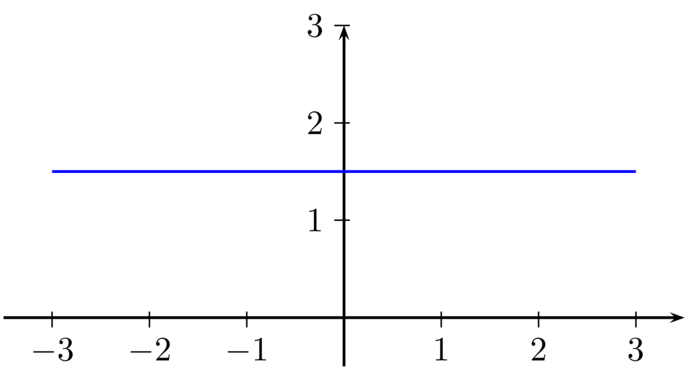
\includegraphics{Picture_FIGLabelFigFoncConstFdDkhWPICTFoncConstFdDkhW-for_eps.pdf}
%The result is on figure \ref{LabelFigFoncConstFdDkhW}.
%\newcommand{\CaptionFigFoncConstFdDkhW}{<+Type your caption here+>}
\input{Fig_FoncConstFdDkhW.pstricks}

\end{multicols}



\begin{wrapfigure}{r}{7.0cm}
   \vspace{-0.5cm}        % à adapter.
   \centering
   \input{Fig_figureCFoZCYe.pstricks}
\end{wrapfigure}

    Sur la figure ci-contre, nous avons tracé les graphes des fonctions données par
    \begin{enumerate}
        \item
            \( f(x)=2x+1\)
        \item
            \( g(x)=2x-2\)
        \item
            \( h(x)=3x-1\)
    \end{enumerate}


Nous constatons que
\begin{enumerate}
    \item
        Les droites représentatives de \( f\) et \( g\) sont parallèles.
    \item
        La droite \( h\) est plus pendue que les deux autres.
\end{enumerate}


\begin{example}
    Soit la fonction \( f(x)=3x-1\).
    \begin{enumerate}
        \item
            Le point \( (0;-1)\) est sur la courbe représentative de \( f\) parce que \( f(0)=1\).
        \item
            Le point \( (10;29)\) est également sur la courbe parce que \( f(10)=29\).
        \item
            Le point \( (2;3)\) n'est par contre pas sur le graphe parce que \( f(2)=5\neq 4\).
    \end{enumerate}
\end{example}

%+++++++++++++++++++++++++++++++++++++++++++++++++++++++++++++++++++++++++++++++++++++++++++++++++++++++++++++++++++++++++++
\section{Petit tour de magie}
%+++++++++++++++++++++++++++++++++++++++++++++++++++++++++++++++++++++++++++++++++++++++++++++++++++++++++++++++++++++++++++

\begin{Aprojeter}
    \begin{example} \label{ExemVmCkIH}
        Un petit tour de magie. Choisissez un nombre entre \( 1\) et \( 10\). Ajoutez \( 5\), multipliez par \( 2\), ajoutez \( 7\), enlevez le double du nombre de départ.
    \end{example}
\end{Aprojeter}

\begin{Aprojeter}
    Pouvez-vous trouver un petit tour de magie qui commence par
    \begin{itemize}
        \item Multiplier par \( 3\)
        \item Faire \( +2\)
        \item \ldots
    \end{itemize}
    et qui donne toujours \( 5\) ?
\end{Aprojeter}

\begin{Aprojeter}
    \lstinputlisting{ex_algo18.py}
\end{Aprojeter}


%+++++++++++++++++++++++++++++++++++++++++++++++++++++++++++++++++++++++++++++++++++++++++++++++++++++++++++++++++++++++++++ 
\section{Ensemble de définition}
%+++++++++++++++++++++++++++++++++++++++++++++++++++++++++++++++++++++++++++++++++++++++++++++++++++++++++++++++++++++++++++

\begin{definition}
    Soit \( \defD\) un ensemble de nombres. On définit une \defe{fonction}{fonction} \( f\) sur \( \defD\) en associant à chaque nombre \( x\) dans \( \defD\) un seul nombre \( y\). Dans ce cas nous disons que \( f\) est une fonction de la \defe{variable}{variable} \( x\).
\end{definition}

\begin{example}
    Soit la fonction qui à la longueur d'un segment fait correspondre la surface du carré construit sur ce segment. Cette fonction n'est définie que sur les nombres positifs (parce qu'il n'existe pas de segments de longueurs négatives). Nous écrivons donc
    \begin{equation}
        \begin{aligned}
            f\colon \mathopen[ 0 , \infty [&\to \eR \\
            x&\mapsto x^2,
        \end{aligned}
    \end{equation}
    et nous avons \( f(x)=x^2\).

    Le symbole \( \mathopen[ 0 , \infty [\) représente l'ensemble de tous les nombres de \( 0\) (y compris) à l'infini, c'est à dire tous les nombres plus grands ou égaux à \( 0\).
\end{example}

\begin{example}
    Soit la fonction qui a un nombre entier fait correspondre la somme de ses chiffres. Par exemple \( f(0)=0\) et \( f(123)=6\). Cette fonction est définie sur les entiers et retourne un entier. Nous pouvons écrire
    \begin{equation}
        \begin{aligned}
            f\colon \eN&\to \eN \\
            x&\mapsto f(x). 
        \end{aligned}
    \end{equation}
    Ici il est compliqué de donner une forme explicite pour \( f\).
\end{example}

\begin{example}
    La fonction carré est :
    \begin{equation}
        \begin{aligned}
            f\colon \eR&\to \eR \\
            x&\mapsto x^2 
        \end{aligned}
    \end{equation}
    Notons que c'est presque la même que la fonction «surface du carré». La différence est le contexte.
\end{example}

\begin{example}
    La fonction racine carré est :
    \begin{equation}
        \begin{aligned}
            \sqrt{}\colon \mathopen[ 0 , \infty [&\to \eR  \\
                x&\mapsto \sqrt{x}. 
        \end{aligned}
    \end{equation}
\end{example}

\begin{example}
    La fonction inverse est :
    \begin{equation}
        \begin{aligned}
            f\colon \eR\setminus\{ 0 \}&\to \eR \\
            x&\mapsto \frac{1}{ x }. 
        \end{aligned}
    \end{equation}
    La notation \( \eR\setminus\{ 0 \}\) représente l'ensemble de tous les nombres sauf zéro.
\end{example}

%--------------------------------------------------------------------------------------------------------------------------- 
\subsection{Intermède : pourquoi ne pas diviser par zéro ?}
%---------------------------------------------------------------------------------------------------------------------------

La fraction \( \frac{1}{ 0.1 }\) est le nombre de fois que \( 0.1\) rentre dans \( 1\). Cela vaut \( 10\) parce qu'il faut \( 10\) soit \( 0.1\) pour faire \( 1\).

Que vaut \( \frac{1}{ 0.0001 }\) ? C'est le nombre de fois que \( 0.0001\) rentre dans \( 1\), c'est à dire dix mille.

Que vaudrait \( \frac{1}{ 0 }\) ? C'est le nombre de fois qu'il faut prendre zéro pour obtenir \( 1\).

\begin{example}
    Considérons la fonction qui a un nombre fait correspondre son inverse : \( f\colon x\mapsto \frac{1}{ x }\). Pour se dérouiller le cerveau, je propose quelque valeurs :
    \begin{equation}
        \begin{aligned}[]
            f(1)&=1&f(5)&=\frac{1}{ 5 }&f(\frac{ 2 }{ 3 })=\frac{ 3 }{ 2 }\\
            f(\frac{ 1 }{ 4 })&=4&f(-3)&=-\frac{1}{ 3 }&f(-1)&=-1.
        \end{aligned}
    \end{equation}
    Cette fonction est implémentée en python de la façon suivante :

\lstinputlisting{ex_inverse.py}

donne

%\lstinputlisting[title=Résultat]{res_ex_inverse.txt}
\VerbatimInput{res_ex_inverse.txt}

Très clairement, python ne veut pas calculer l'inverse de zéro et plante sur un message on ne peut plus clair : \info{ZeroDivisionError: division by zero}.

Effectivement, l'inverse de zéro n'existe pas. L'ensemble de définition de notre fonction \( f(x)=1/x\) n'est donc pas \( \eR\) tout entier, mais seulement \( \eR\setminus\{ 0 \}\).

\end{example}

\begin{Aretenir}        \label{ArtJgipNt}
    Il n'est pas permis de diviser par zéro. Une fonction qui contient un dénominateur ne peut pas avoir dans son ensemble de définition des \( x\) qui annulent le dénominateur. Autrement dit dès que vous voyez
    \begin{equation}
        \frac{1}{ f(x) }
    \end{equation}
    vous devez résoudre l'équation \( f(x)=0\).
\end{Aretenir}

%+++++++++++++++++++++++++++++++++++++++++++++++++++++++++++++++++++++++++++++++++++++++++++++++++++++++++++++++++++++++++++
\section{Antécédent}
%+++++++++++++++++++++++++++++++++++++++++++++++++++++++++++++++++++++++++++++++++++++++++++++++++++++++++++++++++++++++++++

\begin{Aretenir}
Une fonction associe à chaque nombre de l'ensemble de définition \emph{un seul} nombre, appelé \defe{image}{image}. Si \( a\) est un nombre, un \defe{antécédent}{antécédent} de \( a\) par la fonction \( f\) est un nombre \( x\in\defD\) tel que 
\begin{equation}
    f(x)=a.
\end{equation}
Autrement dit, les antécédents de \( a\) sont les éléments de \( \eR\) dont l'image par \( f\) est \( a\).

Il peut arriver qu'un nombre ait plusieurs antécédents.
\end{Aretenir}


\begin{example}
    Pour la fonction \( f(x)=2x-1\), un antécédent de \( 5\) est le nombre \( 3\). Un antécédent du nombre \( -10\) est la nombre \( -9/2\).
\end{example}

\begin{Aretenir}
    Trouver les antécédents de \( a\) par la fonction \( f\) revient à trouver les solutions de l'équation
    \begin{equation}
        f(x)=a.
    \end{equation}
\end{Aretenir}


\begin{example}

    Les antécédents de \( 4\) pour la fonction \( f(x)=2x-1\) sont les solutions de l'équation
    \begin{equation}
        2x-1=4
    \end{equation}
    c'est à dire \( x=\frac{ 5 }{2}\). Il se fait qu'il y en a un seul.

    Plus généralement l'antécédent de \( a\) pour cette fonction est la solution de l'équation
    \begin{equation}
        2x-1=a,
    \end{equation}
    c'est à dire le nombre \( x=\frac{ a+1 }{ 2 }\).
\end{example}

\begin{example} \label{EqlaIGDz}
    Si nous avons une série statistique de \( n\) valeurs, pour trouver le premier quartile nous devons diviser \( n\) par \( 4\) et prendre l'entier le plus proche vers le haut. Cela donne le numéro de la valeur correspondante au premier quartile.

    En python, la fonction qui donne le numéro de la valeur du premier quartile en fonction de \( n\) est
    \begin{quote}
        \info{math.ceil(n/4)}
    \end{quote}
    Notons \( f\) cette fonction. Son ensemble de définition est l'ensemble des entiers non nuls. Le graphique de cette fonction est donné à la figure \ref{LabelFigMathCeilwCXIJZ}.
\newcommand{\CaptionFigMathCeilwCXIJZ}{Le numéro de la valeur du premier quartile en fonction du nombre de valeurs.}
\input{Fig_MathCeilwCXIJZ.pstricks}

    Le graphique est uniquement constitué de points. Pas de lignes entre, parce qu'il n'existe pas de séries statistiques comprenant \( 3.7\) valeurs par exemple. 
\end{example}

\Exo{Seconde-0053}

\begin{example}
    Soit la fonction \( f(x)=(x+1)^2\). Nous avons \( f(-1)=0\), \( f(4)=25\); nous disons que \( 0\) est l'image de \( -1\) par \( f\) et que \( 25\) est l'image de \( 4\) par \( f\).

    Remarquons que \( f(-2)=1\) et \( f(0)=1\). Donc \( -2\) et \( 0\) sont deux antécédents de \( 1\).
\end{example}

\begin{example}
    Le nombre \( 4\) est un antécédent de \( 3\) pour la fonction \( f(x)=\frac{ x }{ 2 }+1\).
\end{example}

\begin{example}
    Les nombres \( 3\) et \( -3\) sont tout deux des antécédents de \( 9\) pour la fonction \( x\mapsto x^2\).
\end{example}

